%======================================================================
\chapter{Introduction}
%======================================================================

Our world-wide Increasing population and standard of living has lead to an increasing demand for basic human needs such as food and energy, putting significant pressure on sectors such as agriculture, energy production etc. The International Energy Outlook has made a forecast of a 48\% rise in global energy consumption from 549 to 815 quadrillion BTU between 2012 and 2040 \cite{}. The unprecedented level of fossil fuels required to be burnt for this much energy production is simply alarming for two reasons, first the catastrophic environmental impacts ,and second fossil fuels are a finite resource. So the world urgently requires stable and consistent clean energy technology.

Solar energy is a clean alternative to fossil fuel, that has received considerable academic, political, and industrial interest in recent years. Harnessing energy through the use of solar panels is one of the most affordable clean energy technologies that has been developed. However, the electricity per unit cost from solar power is still quite high as compared to conventional sources making it unaffordable for wide-spread use. The major limitation is material cost, and process quality. Thus, further research is required to develop cheaper technologies that are able to create efficient yet durable solar cells.

\section{Materials requirements for photovoltaic application}

A solar cells is an electrical device than converts light energy into electrical energy via the photovoltaic effect in which electron flow is generated by absorbing photons. They are produced from thin slices or wafers of a suitable material. Semiconductors are perfect for this application since their band gap lies in the visible spectrum (1.5 eV) and release electrons on absorbing solar energy. 

% Flow of electrons requires energy for electrons to jump from top of valance band to conducting band. This energy difference is band gap

%The wafer material is also required to have good quantum efficiency. Quantum efficiency is the ratio of photons falling on the surface of the material and the electricity generated from it. Among many factors, this is also dependent on the minority carrier concentration and lifetime. Minority carriers are electron and hole pairs flowing inside the semiconductors that are generated on absorbing energy greater than the band gap. Minority carrier lifetime can be reduced by the defects present inside material such as dislocations, grain boundary, precipitates etc. So a defect free crystalline material has good quantum efficiency and thus, serves as a wafer material.

In order to be a good solar cell, the wafer material is required to have good efficiency in terms of the quantity of electricity produced for a given amount of light. Among many factors, this is also dependent on the defects present inside the material such as dislocations, grain boundary, and impurity atoms to name a few. Crystalline materials that are defect-free fit this description, but are very costly to produce. The material should also have good mechanical strength in order to withstand the wafer development process and final deployment in external environments. To save costs, wafers are produced at a thickness of 200-400 microns. At such thicknesses, the chance of breaking via brittle fracture increases significantly. The mechanical properties of the material also influence surface crack formation during the sawing process, which affects the final strength of the wafers \cite{}. A material with good mechanical properties is therefore imperative for the production of durable solar cells.

\section{Silicon as a photovoltaic material}
Silicon is widely used to make solar cell wafers. It is used, among all semiconductors, because it is a very abundant material on earth and being a widely used electronic material, its physical and chemical properties have already been well-studied. Several technologies such as Chozarlaski and Float-zone process already exist to produce mono-crystalline silicon (c-Si) at industrial scale. It should be noted that there are materials such as CdTe (1.49 eV) and GaAs (1.43 eV) with band gap closer to the visible spectrum (1.5 eV), but silicon (1.1 eV) is used over them because it is more economical to produce it industrially.


Silicon is produced through first extraction from silica and then purified for wafer fabrication. The silicon extracted from silica is 98\% pure, and is referred to as metallurgical grade silicon (MGS). This is used for many different applications, most notably as an alloying element in aluminum alloy products. Silicon used for electronic applications, referred to as electronic grade silicon (EGS), requires additional purity, up to 99.99\% pure. The purification of MGS into EGS is accomplished using the Chozarlski or Float-zone processes, which achieve not only high purity but also result in c-Si. Initially, EGS was used for solar cell wafer fabrication. These c-Si ingots were then sliced into wafers via wire sawing. These processes are, however, very expensive and lead to an increase in final cost of solar panels. Additionally, the material is of higher purity that is actually required for solar applications.

In recent years, research on producing solar grade silicon (SGS) has focused on directlonal solidification (DS) of the MGS material to directly create SGS. However, DS produces multi-crystalline silicon (mc-Si) ingots instead of c-Si ingots which leads to efficiency loss due to the presence of grain boundaries and a higher level of dislocations.  Apart from that, mc-Si ingots are usually contaminated with impurities such as O, Fe, Cr, Ni, Ti and Cu which further lead to efficiency loss \cite{davis1980impurities,coletti2011impact} . These impurities are incorporated from the crucible during DS process \cite{istratov2003metal} or can be already present in the feedstock. So a cost saving in producing ingots through DS process comes at an efficiency loss in the solar cells. However, this loss in efficiency can be reduced by efficiently changing the parameters used during DS and wire sawing processes.

PRISED solar, a company based in Toronto, has developed a purifying method to upgrade the MGS into SGS. This involves migration of impurities to internal surfaces using microwave and trapping them into neutral sites using gettering agents. This purification is done on a wafer or pellet geometry. These wafers can be made from wire sawing of MGS ingots made via directional solidification process. 

\section{Directional solidification}
It has been found that grain boundaries and grain boundary orientations have a significant affect on the efficiency of mc-Si solar cells \cite{fujiwara2006directional}. DS process is a solidification process which facilitates reduction of grain boundary by development of large grains inside the solid. Therefore, DS process is used industrially for producing mc-Si blocks and ingots for development of solar cells.

\noindent
\begin{minipage}[c]{\textwidth}
\centering
        \captionsetup{type=figure}
        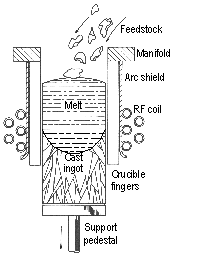
\includegraphics[width=3.0in]{EMcasting.png}
        \captionof{figure}{Directional Solidification}
        \label{fig:DS}
 \end{minipage}
 
DS process is achieved by a uni-directional extraction of heat from the melt which leads to a planer movement of solid-liquid interface. As shown in Figure\ref{fig:DS}, MGS is provided as feedstock for DS and converted into molten silicon. Heat is then extracted from the bottom surface only, while the other surfaces are insulated to ensure a planer solidification front. The use of DS has an additional advantage in that it will further purify the feedstock through a process known as segregation.

Segregation is the phenomenon of separating a constituent from the forming solid phase via rejection into the melt. The amount of segregation is measured by the segregation coefficient, $k_{0}$
  \[k_{0}=\frac{C_{S}}{C_{L}} \]
where, $C_{S}$ and $C_{L}$ are the constituents' concentration in the solid and liquid phases, respectively. For most metals constituents in silicon, $k_{0}<1$ which means the impurity prefers to stay in the liquid. As solidification within an ingot reaches completion, the impurities concentrate at the top as it is the last part to solidify. This process be be repeated several times to further segregate and remove impurities. The part left behind once the impure part has been removed is used as SGS feedstock for wafer fabrication.  

The rate of cooling is an important parameter during DS. As a slow cooling rate lead to large grain sizes and thus less grain boundary area, it is preferred over a faster cooling. But a slow cooling rate also comes at increased manufacturing time and cost. The rate of cooling during DS also determines the level and the distribution of dislocations formed inside the solid \cite{moller2005multicrystalline, ryningen2011growth}. A faster cooling rate leads to a higher dislocation density due to strain from differential thermal expansion between top and bottom of the ingot. The rate of cooling is therefore a very crucial factor during DS process.

\section{Wafer production by Wire sawing}
SGS ingots from the DS process are converted into solar wafers via sawing techniques. Among the many sawing techniques, multi wire sawing is the most efficient since it can be used to cut all of the ingot at once. 80\% of the SGS wafers produced industrially use multi wire sawing \cite{}. During wire sawing, SGS ingots are glued to a substrate holder and placed in a wire saw which then slices them into thin wafers. This process is shown in Figure \ref{fig:wire-saw}. As can be seen, a single wire is fed from a supply spool through a pulley and tension control unit to four wire guides. The SGS ingot on the holder is pushed down the wire web which leads to material removal and slicing. This wire is under tension during this process, and may be at different levels of strain depending on the depth of the cut.  
\begin{figure}[ht]
    \centering
    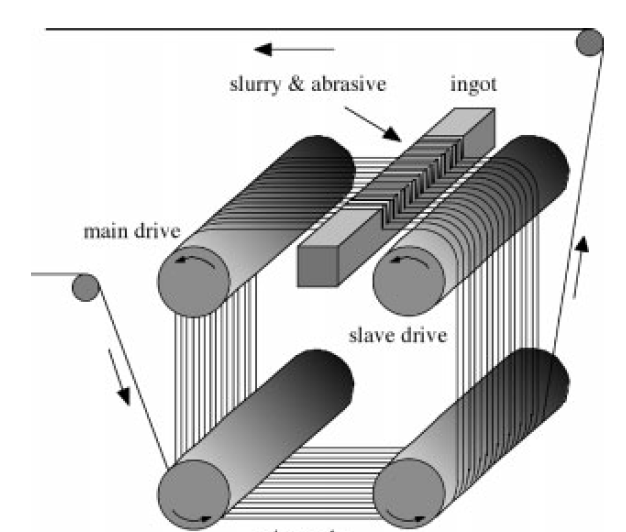
\includegraphics[width=3.0in]{wire-saw.PNG}
    \caption{figure}{Wire Sawing Setup}
    \label{fig:wire-saw}
\end{figure}
The wire is made of stainless steel and has a typical diameter of around 150-200 micron. The volume between the wire and the ingot surface is covered with slurry containing abrasives such as SiC and diamond particles. The size of these abrasive particles are around 5-30 micron \cite{}. The slurry moves with the movement of the wire and acts as a transport medium for the abrasives into the sawing channels. The slurry has to be highly viscous and so usually made out of oil or ethyl alcohol. The slurry also must minimize temperature rise during wire sawing by continually removing the heat of cutting. The actual material removed, also known as Kerf loss, is around 200-250 microns per wafer. Thus, the kerf loss is nearly 50\% of total wafer material. This wastage of material makes wire sawing an expensive method.
\newline
\noindent
\begin{minipage}[c]{\textwidth}
\centering
        \captionsetup{type=figure}
        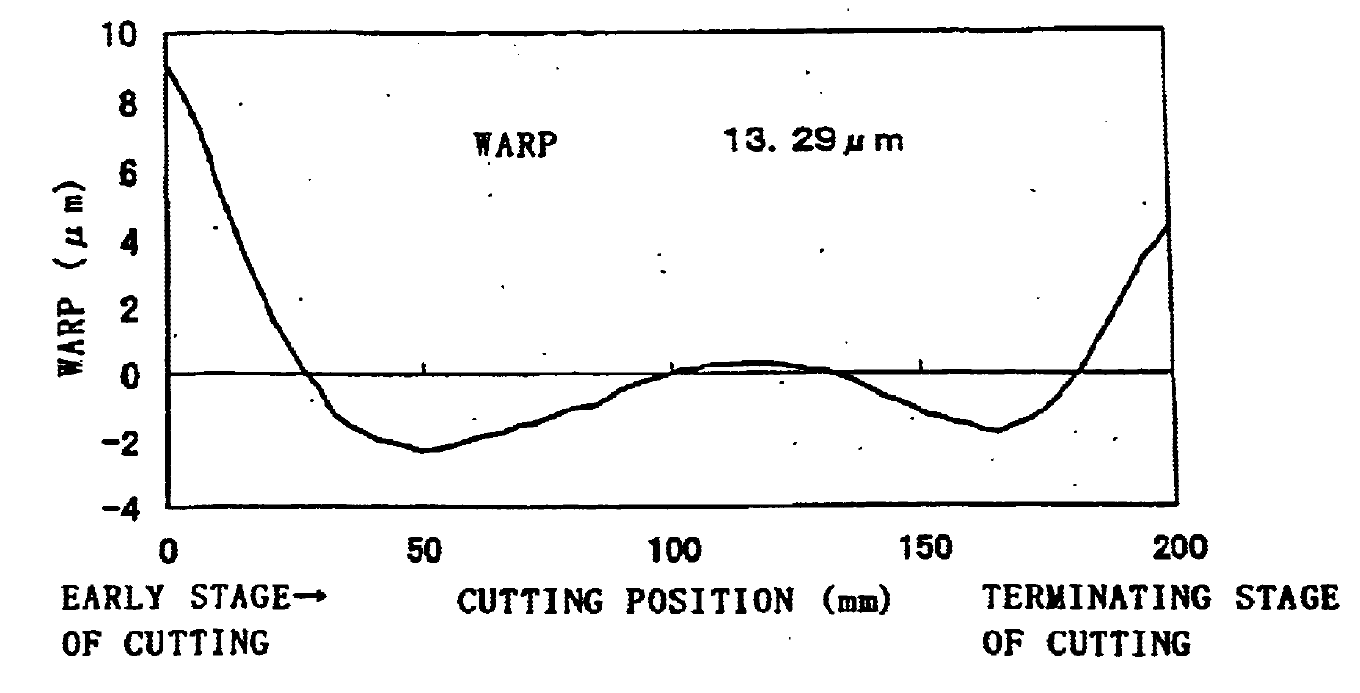
\includegraphics[width=5.0in]{observed-warpage.PNG}
        \captionof{figure}{Warpage in wafers \cite{}}
        \label{fig:warpage}
 \end{minipage}
 
Although wire sawing is an efficient process, the wafer produced can be non flat i.e. have warpage in it as shown in Figure \ref{fig:warpage}. This occurs due the development of thermal gradients between different locations in the work piece during sawing. The amount of warpage depends upon the wire sawing parameters such as wire speed, tension etc and the work piece properties such as residual stress. Warpage in wafers is undesirable as it creates a difficulty during fabrication of solar cells, and reduced photovoltaic efficiency. 

\section{Summary}
Wafers for solar cells are made from SGS material through a multi step process involving DS of mc-Si ingots and wire sawing of these ingots. During these processes, defects such as warpage, dislocations, and residual stresses can be induced in the final wafer which increases component costs and reduces the efficiency of the solar cells. In this thesis, a mathematical model for simulating the dislocation density, residual stress and warpage during processing is developed that can be used to understand the link between processing and solar cell wafer performance. In the next chapter, prior research conducted in the area of numerical simulation of directional solidification and wire sawing, along with the theories developed for predicting the thermoplastic behaviour of silicon are reviewed.